\documentclass[14pt]{extreport}
\usepackage{gost}
\usepackage{lscape}
\usepackage{multirow}
% объявляем новую команду для переноса строки внутри ячейки таблицы
\newcommand{\specialcell}[2][c]{%
  \begin{tabular}[#1]{@{}c@{}}#2\end{tabular}}



\begin{document}
\begin{figure}[]
		
\includegraphics[scale=0.66]{itmo_image.png}
		\label{pic1}
\end{figure}
\begin{flushleft}
\begin{tabular}{ p{9cm}p{8cm} }
 Группа: K3120 & К работе допущен: \\ 
 Студент: Скворцов И.В. & Работа выполнена: \\  
 Преподаватель: Попов А. С. & Отчет принят: \\    
\end{tabular}
\end{flushleft}

\begin{center}
\Large\textbf{Рабочий протокол и отчёт по\\лабораторной работе №1.05}

\large\textbf{Исследование колебаний физического маятника}
\end{center}

\section*{1. Цель работы.}

\begin{enumerate}
    \item Изучение характеристик затухающих колебаний физического маятника. 
\end{enumerate}

\section*{2. Задачи.}
\begin{enumerate}
    \item Измерение периода затухающих колебаний.
    \item Определение зависимости амплитуды затухающих колебаний физического маятника от времени.
    \item  Определение зависимости периода колебания от момента инерции физического маятника
    \item Определение преобладающего типа трения
    \item Определение экспериментальной и теоретической приведенных длин маятника при его разных конфигурациях
\end{enumerate}

\section*{3. Объект исследования}
Физический маятник и его колебания

\section*{4. Метод экспериментального исследования.}
Эмпирический лабораторный экспериментальный

\section*{5. Рабочие формулы и исходные данные.}
Среднее время колебаний 
\begin{equation}\label{f1}
   \overline{t} = \frac{1}{3} (t_1 + t_2 + t_3)
\end{equation}

Средний период колебаний
\begin{equation}\label{f1}
   T = \frac{\overline{t}}{N}
\end{equation}

Циклическая частота затухающих колебания
\begin{equation}\label{f1}
   \omega = 2\pi v = \frac{2\pi}{T}
\end{equation}

Соотношение циклической частоты затухающих колебаний с циклической частотой собственных колебаний, оттуда циклическая частота собственных колебаний
\begin{equation}\label{f1}
   \omega = \sqrt{\omega_{0}^2 - \beta^2}
\end{equation}

\begin{equation}\label{f1}
   \omega = \sqrt{\omega^2 + \beta^2}
\end{equation}

Логарифмический декремент колебаний с коэффициентом затухания и периодом затухающих колебаний

\begin{equation}\label{f1}
   \lambda = \ln{\frac{A(t)}{A(t + T)}} = \beta t
\end{equation}

\section*{6. Измерительные приборы}
\begin{table}[H]\label{t1}
\caption{Измерительные приборы.}
\centering
\begin{tabular}{|c|c|c|c|c|}
\hline
 № и/п & Наименование & Тип прибора & Используемый & Погрешность \\ 
 & & & диапазон & прибора \\ \hline
 1 & Шкала & Цифровой & [0; 25] $^\circ$ & 1 $^\circ$ \\ \hline
 2 & Секундомер цифровой & Цифровой & [0; 3600], с & 0.0005, с \\ \hline
 
\end{tabular}
\end{table}

\section*{7. Схема установки}
\begin{figure}[H]
	\begin{center}
		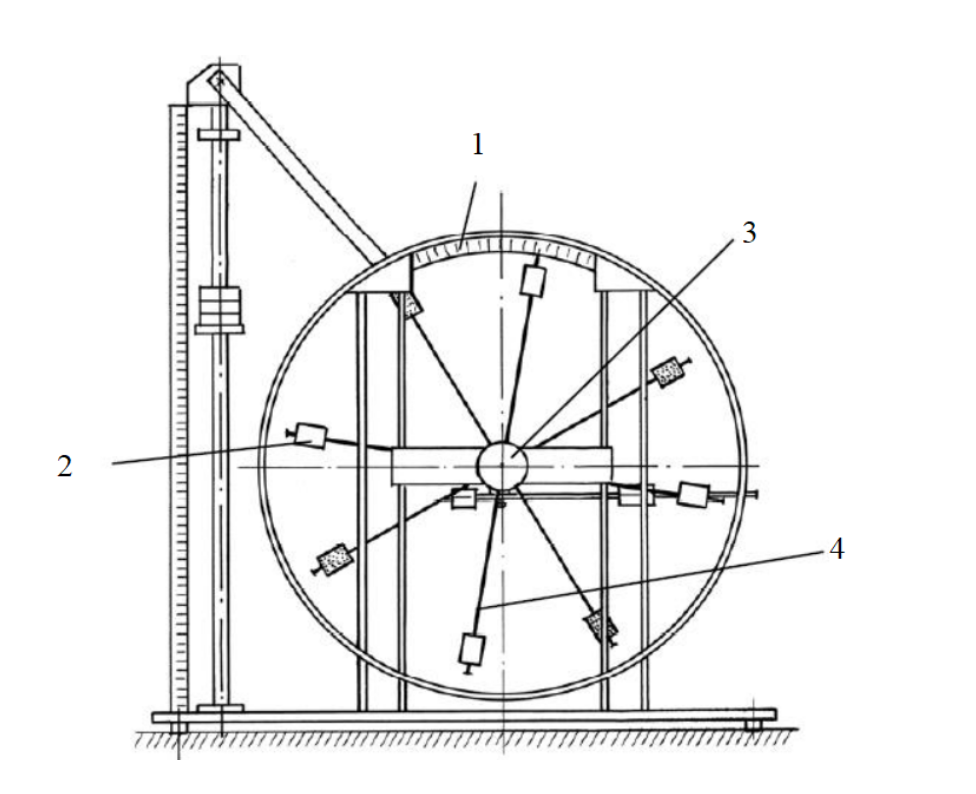
\includegraphics[scale=0.7]{Scheme.png}
		\caption{Схема экспериментальной установки}
		\label{pic}
	\end{center}
\end{figure}

\newpage
\section*{8. Результаты прямых измерений и их обработка.}
\begin{table}[!h]
    \centering
    \begin{tabular}{|l|l|l|l|l|l|}
    \hline
        Угол отклонения & 5 & 10 & 15 & 20 & 25  \\ \hline
        $t_1, c$ & 44.07 & 91.18 & 148.73 & 215.04 & 300.19  \\ \hline
        $t_2, c$ & 44.35 & 88.91 & 146.22 & 212.49 & 298.94  \\ \hline
        $t_3, c$ & 41.95 & 91.08 & 146.14 & 214.51 & 300.93  \\ \hline
        $\overline{t}$, c & 43.46 & 90.39 & 147.03 & 214.01 & 299.565 \\ \hline
    \end{tabular}
    \caption{Значения времени 10 колебаний в зависимости от угла отклонения}
\end{table}


\begin{table}[!h]
    \centering
    \begin{tabular}{|l|l|l|l|l|l|}
    \hline
        Положение боковых грузов & $t_1$ & $t_2$ & $t_3$ & $\overline{t}$ & T  \\ \hline
        1 риска & 16.81 & 16.31 & 16.36 & 16.49 & 1.649  \\ \hline
        2 риска & 17.46 & 17.11 & 17.31 & 17.29 & 1.729  \\ \hline
        3 риска & 18.61 & 18.46 & 18.35 & 18.47 & 1.847  \\ \hline
        4 риска & 19.85 & 20.06 & 20.01 & 19.97 & 1.997  \\ \hline
        5 риска & 20.91 & 21.21 & 20.96 & 21.02 & 2.102  \\ \hline
        6 риска & 22.36 & 22.35 & 22.51 & 22.41 & 2.241 \\ \hline
    \end{tabular}
    \caption{Значение времени 10 колебания и периода колебания в зависимости от положения грузов}
\end{table}

\newpage


\section*{9. Расчет результатов косвенных измерений.}

1) Из графика зависимости A от t видно, что в нашем случае имеет место быть сухое трение. 

2) С помощью метода наименьших квадратом найдем коэффиценты зависимости
$A(t) = A_0 + kt$

\begin{center}
    $k = -0.08$ \\ 
    $A_0 = 27.32^\circ $
\end{center}

3) Найдем ширину зоны застоя и оценим, через сколько периодов колебания прекратятся.

\begin{center}
    $\Delta \varphi_{3} = \frac{A_0 - A(NT)}{4N}$ \\
    $\Delta \varphi_{3} = 0.032$ \\
    $N = \frac{\Delta \varphi_{з} - A_0}{kT}$ \\
    $N = 212,16 $
\end{center} 

4) По угловому коэффиценту графика $T^2(I)$ найдем произведение ml

\begin{center}
    $ml = \frac{4\pi^{2}I}{gT^2} = 0.17$
\end{center}

5) Рассчитаем $l$(пр эксп) и $l$(пр эксп), внесем результаты в таблицу 4

\begin{table}[!ht]
    \centering
    \begin{tabular}{|l|l|l|l|l|l|l|}
    \hline
        Риски & 1 & 2 & 3 & 4 & 5 & 6  \\ \hline
        $R_\text{верх}$, м & \multicolumn{6}{c|}{0.08}   \\ \hline
        $R_\text{ниж}$, м & \multicolumn{6}{c|}{0.202}   \\ \hline
        $R_\text{бок}$, м & 0.077 & 0.102 & 0.127 & 0.15 & 0.18 & 0.202  \\ \hline
        $I_\text{гр}$, кг*м$^2$ & 0.096 & 0.1102 & 0.129 & 0.15 & 0.18 & 0.209  \\ \hline
        $I$, кг*м$^2$  & 0.104 & 0.118 & 0.137 & 0.16 & 0.19 & 0.217  \\ \hline
        $l_\text{пр эксп}$, м & 0.68 & 0.74 & 0.85 & 0.99 & 1.096 & 1.25  \\ \hline
        $l_\text{пр теор}$, м & 0.802 & 0.86 & 0.93 & 1.016 & 1.117 & 1.228 \\ \hline
    \end{tabular}
    \caption{Результаты расчетов косвенных измерений}
\end{table}
Пример расчетов:

\begin{center}
    $R_\text{верх}$ $= l_1 + (n-1)l_0 + 0.5b = 0.057 + (1 - 1)*0.025 + 0.5 * 0.04 = 0.077$ м \\
    $R_\text{ниж}$ $= l_1 + (n-1)l_0 + 0.5b = 0.057 + (6 - 1)*0.025 + 0.5 * 0.04 = 0.202$ м \\
    $I_\text{гр}$ $=m_\text{гр}(R_\text{верх}^2 + R_\text{ниж}^2 + R_\text{бок}^2)=$\\$ 1.632(0.077^2 + 0.202^2 + 2*0.077^2) = 0.096$ кг*м$^2$ \\
    $I = I_0 + I_\text{гр} = 0.008 + 0.096 = 0.104$ кг*м$^2$ \\
    $l_\text{пр эксп} = \frac{T^2 * g}{4\pi^2} = \frac{1.649^2 * 9.8}{4\pi^]} = 0.68$ м \\ 
     $l_\text{пр эксп}  = l_\text{теор} + \frac{I}{m_\text{гр}*l_\text{теор}} = 0.104 + \frac{0.104}{4*0.408 * 0.104} = 0.802$ м
\end{center}

\newpage


\section*{10. Графики}

\begin{figure}[H]
	\begin{center}
		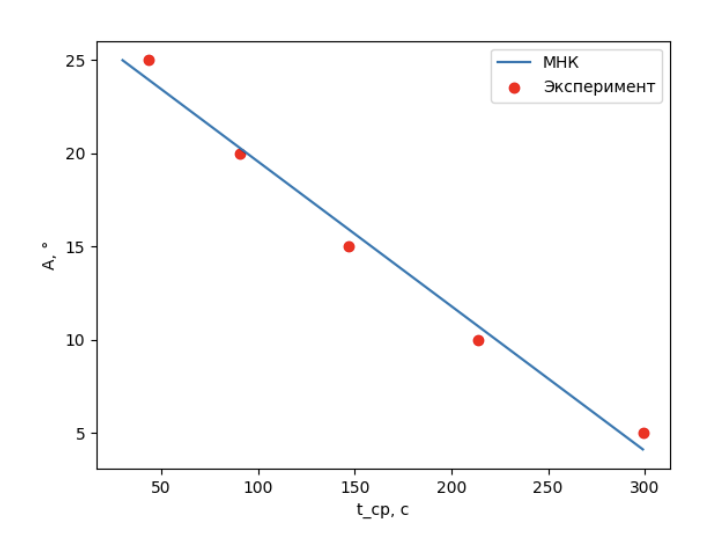
\includegraphics[scale=0.8]{A_t.png}
		\caption{График зависимости A(t)}
		\label{pic}
	\end{center}
\end{figure}

\begin{figure}[H]
	\begin{center}
		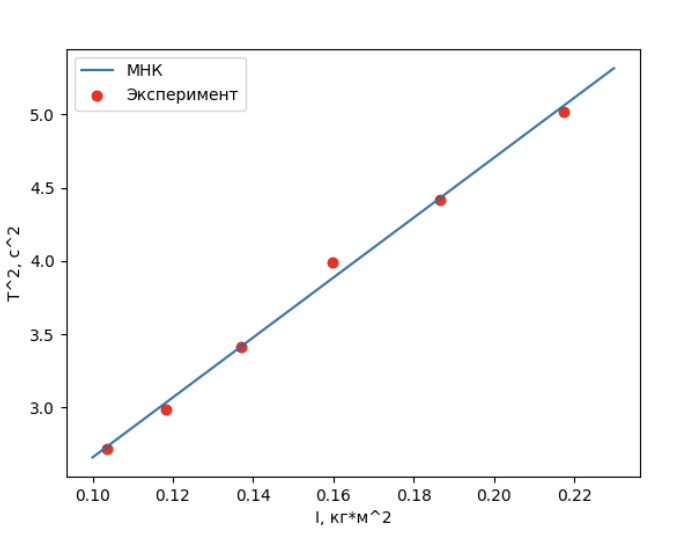
\includegraphics[scale=0.9]{T_I.png}
		\caption{График зависимости $T^2(I)$}
		\label{pic}
	\end{center}
\end{figure}

\newpage

\section*{11. Окончательные результаты}
\begin{table}[!h]
    \centering
    \begin{tabular}{|l|l|l|l|l|l|l|}
    \hline
        Риски & 1 & 2 & 3 & 4 & 5 & 6  \\ \hline
        $l_\text{пр эксп}$, м & 0.68 & 0.74 & 0.85 & 0.99 & 1.097 & 1.25  \\ \hline
        $l_\text{пр теор}$, м & 0.802 & 0.86 & 0.928 & 1.016 & 1.117 & 1.228 \\ \hline
    \end{tabular}
    \caption{Результаты расчетов $l_\text{пр эксп}$ и $l_\text{пр теор}$}
\end{table}


\section*{12. Выводы и анализ результатов работы}

В данной лабораторной работе мы исследовали характеристики затухающих колебаний физического маятника. В ходе обработки результатов было определено, что в рассматриваемом эксперименте преобладает сухое трение. Кроме того, были посчитаны величины $l_\text{пр эксп}$ и $l_\text{пр теор}$, которые оказались примерно равны. 


\end{document}

